\documentclass[11pt,twoside]{scrartcl}
%\documentclass[11pt,twoside]{article}

%opening
\newcommand{\lecid}{15-316}
\newcommand{\leccourse}{Software Foundations of Security and Privacy}
\newcommand{\lecdate}{} %e.g. {October 21, 2013}
\newcommand{\lecnum}{8}
\newcommand{\lectitle}{Control Flow Safety}
\newcommand{\lecturer}{Matt Fredrikson}
\newcommand{\lecurl}{https://15316-cmu.github.io/index}

\usepackage{varwidth}
\usepackage{lecnotes}
\usepackage[irlabel]{bugcatch}

\usepackage{tikz}
\usetikzlibrary{automata,shapes,positioning,matrix,shapes.callouts,decorations.text,patterns,trees,backgrounds}

% \usepackage[bracketinterpret,seqinfers,sidenotecalculus]{logic}
% \newcommand{\I}{\interpretation[const=I]}

% \newcommand{\bebecomes}{\mathrel{::=}}
% \newcommand{\alternative}{~|~}
% \newcommand{\asfml}{F}
% \newcommand{\bsfml}{G}
% \newcommand{\cusfml}{C}
% \def\leftrule{L}%
% \def\rightrule{R}%

\begin{document}

\newcommand{\atrace}{\sigma}%
%% the standard interpretation naming conventions
\newcommand{\stdI}{\dTLint[state=\omega]}%
\newcommand{\Ip}{\dTLint[trace=\atrace]}%
\newcommand{\ws}{\omega}\newcommand{\wt}{\nu}% 

\maketitle
\thispagestyle{empty}

%%%%%%%%%%%%%%%%%%%%%%%%%%%%%%%%%%%%%%%%%%%%%%

\section{Introduction \& Recap}

In the last lecture we talked about enforcing a more granular type of memory safety policy to ensure that parts of our program don't read or write portions they aren't supposed to. This was motivated by our hypothetical career as an app developer who wants to monetize with advertising, and is thus compelled by Vladimir's discount ad shop to run untrusted rendering code within our program:
\[
\pif{\textit{display ads}}{\asprg}{\textit{continue without ads}}
\]
We discussed sandboxing policies where a region of memory is designated for the untrusted $\asprg$ to ``play'' in, such as the upper portion of memory at addresses 8-15 in the diagram below.
\begin{center}
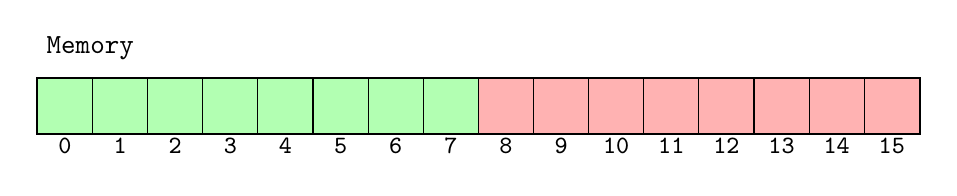
\begin{tikzpicture}[%
    arraynode/.style={
        draw,
        node contents={[\the\numexpr\pgfmatrixcurrentrow-2\relax][\the\numexpr\pgfmatrixcurrentcolumn-2\relax]},
        alias=n\the\numexpr\pgfmatrixcurrentrow-2\relax\the\numexpr\pgfmatrixcurrentcolumn-2\relax
        },
    columnlabel/.style={
        minimum size=0pt,
        draw=none,
        red,
        node contents={\the\numexpr\pgfmatrixcurrentcolumn-2\relax},
        alias=c\the\numexpr\pgfmatrixcurrentcolumn-2\relax
        },      
    rowlabel/.style={
        minimum size=0pt,
        draw=none,
        red,
        node contents={\the\numexpr\pgfmatrixcurrentrow-2\relax},
        alias=r\the\numexpr\pgfmatrixcurrentrow-2\relax
        },      
    emptynode/.style={node contents=~, draw=none},
    font=\ttfamily,
    array/.style={%
        matrix of nodes,
        nodes = arraynode,
        column sep=-\pgflinewidth,
        row sep=-\pgflinewidth, 
        nodes in empty cells,
        row 1/.style={nodes=columnlabel},
        column 1/.style={nodes=rowlabel},
        row 1 column 1/.style={%
            nodes=emptynode}}, 
    rowlabel2/.style={
        inner sep=2pt,
        draw=none,
        font=\small\ttfamily,
        node contents={\the\numexpr-1+\pgfmatrixcurrentcolumn\relax},
        alias=m\the\numexpr-1+\pgfmatrixcurrentcolumn\relax
        },      
    memoryrow/.style={%
        matrix of nodes,
        row 1/.style={nodes = {draw, minimum size=7mm}},
        column sep=-\pgflinewidth,
        row sep=-\pgflinewidth, 
        nodes in empty cells,
        row 2/.style={nodes=rowlabel2}}, 
    memory/.style={%
        matrix of nodes,
        nodes={draw, minimum size=6mm, anchor=center},
        row 1/.style={nodes = {columnlabel, black}},
        column 1/.style={nodes = {rowlabel, black}},
        row 1 column 1/.style={nodes = emptynode},
        column sep=-\pgflinewidth,
        row sep=-\pgflinewidth, 
        nodes in empty cells,
    } 
]

\begin{scope}[yshift=-4cm]

\matrix[memoryrow] (memrow) {
&&&&&&&&&&&&&&&\\
&&&&&&&&&&&&&&&\\};

\node[above right=1mm and 0 of memrow-1-1.north west] {Memory};
\draw[thick] (memrow-1-1.north west) rectangle (memrow-1-16.south east);

\begin{scope}[on background layer]
\fill[red!30] (memrow-1-9.north west) rectangle (memrow-1-16.south east);
\fill[green!30] (memrow-1-1.north west) rectangle (memrow-1-8.south east);
\end{scope}
\end{scope}

\end{tikzpicture}
\end{center}
As long as we can enforce this policy, and we are careful about writing our program to save and restore variable state, then we can ensure that whatever the sandbox does will not affect the rest of our program's execution.

We discussed an approach called \emph{software fault isolation}~\cite{Sehr2010,Yee2009} (SFI) for properly isolating the malicious or buggy effects of $\asprg$ from the rest of our program. SFI works by inlining enforcement directly into $\asprg$, changing its behavior so that it can't violate the sandbox policy and if it attempts to do so then it still won't have any effect on the rest of our execution. SFI is a very practical technique, and has been used effectively in real applications to isolate untrusted code execution from browsers, operating systems, and other critical applications. In the next lab, you will implement a prototype SFI policy for your server.

Today we will look at a related technique called \emph{control flow integrity}~\cite{Abadi2009}, which ensures that the attacker cannot influence the control flow of a program to diverge from a pre-defined control flow policy. But in order for this defense to have any purpose, we need to introduce indirect control flow commands into our language, bringing it closer yet to the features that real platforms in need of rigorous security defenses have in practice. We will then generalize the safety enforcement techniques discussed so far, introducing a flexible and practical method for enforcing safety policies provided as \emph{security automata}~\cite{Schneider2000}.


\section{Indirect control flow}
So far the programs that we have considered have a particularly nice property. Namely, once the programmer decides which commands are in the program and how they are sequenced together with compositions, conditionals, and while loops, then all of the possible sequences of commands that the program will ever execute are fixed once and for all. There is no way for a user to provide data that could cause some of the commands to be skipped over or added, and as long as the program is executed faithfully to the semantics, the control flow will be as the programmer envisioned when the program was written.

Programs executed on ``real'' machines do not enjoy this property, thanks to indirect transfers of control flow. An indirect control flow transfer is commonly implemented using a function pointer in high-level languages, or a \verb'jmp' instruction with a pointer operand. We'll add this functionality to our language by considering a program command of the form:
\begin{equation}
\label{eq:ifjump}
\pifjump{\ivr}{\astrm}
\end{equation}
The command in (\ref{eq:ifjump}) first tests whether a formula $\ivr$ is true in the current state. If it is, then control transfers to the instruction indexed by the term $\astrm$. Otherwise, control proceeds to the next instruction.

But this doesn't make much since yet, because we haven't discussed indexing of instructions. Programs in the simple imperative language are themselves just commands, which can be built from other commands by connecting them with composition, conditional, and looping constructs. We will now change the language so that rather than having structured high-level commands like $\pif{\ivr}{\asprg}{\bsprg}$ and $\pwhile{\ivr}{\asprg}$, we will assume that programs are sequences of unstructured ``atomic'' commands. So the commands are defined by the syntax:
\begin{equation*}
  \asprg ~\bebecomes~
  \pupdate{\pumod{x}{\astrm}}
  \alternative
  \pupdate{\pumod{\pderef{\astrm}}{\bstrm}}
  \alternative
  \passert{\ivr}
  \alternative
  \pifjump{\ivr}{\astrm}
\end{equation*}
Then a program $\Pi$ is a finite sequence of commands,
\begin{equation}
\Pi = (\asprg_0,\asprg_1,\ldots,\asprg_n)
\end{equation}
We will write $\Pi(i)$, where $0 \le i \le n$, to refer to the command $\asprg_i$ in program $\Pi$. If $i$ is negative, or $n < i$, then $\Pi(i)$ is undefined.

Think of this language as a simplified version of assembly language. Memory update commands $\pumod{\pderef{\astrm}}{\bstrm}$ correspond to store instructions (i.e., \verb'mov' into a memory cell), memory dereference terms $\pderef{\astrm}$ correspond to memory fetch instructions (i.e., \verb'mov' from a memory cell to a register), and $\pifjump{\ivr}{\astrm}$ to conditional \verb'jmp' instructions. We don't have an explicit stack or notion of procedure to worry about, but if we did then $\phalt$ commands would correspond to \verb'ret' instructions.

\paragraph{Semantics.}
Recall that program states $\omega$ are composed of a variable map $\omega_V$ and memory $\omega_M$. Now that programs $\Pi$ are composed of indexed commands, and can transfer control to any command in $\Pi$, states will also need to track a program counter $\omega_i$ that determines which command executes next. The program counter will range from $i \in 0$ to $n$, denoting that the command $\Pi_i$ executes next.

\begin{definition}[Operational semantics of programs]
The small-step transition relation $\smallstep_\Pi$ of program $\Pi$ composed of commands $\asprg_0,\ldots,\asprg_n$ in state $\omega = (\omega_i,\omega_V,\omega_M)$ is given by the following cases:
\[
(\omega_i,\omega_V,\omega_M) \smallstep_\Pi
\left\{
\begin{array}{lcl}
(\omega_i+1, \memupd{\omega_V}{x}{\omega\llbracket\astrm\rrbracket}, \omega_M) & \textit{if} & \Pi_i = \pumod{x}{\astrm}~\text{and}~\omega\llbracket\astrm\rrbracket~\text{is defined}

\\

(\omega_i+1, \omega_V, \memupd{\omega_M}{\omega\llbracket\astrm\rrbracket}{\omega\llbracket\bstrm\rrbracket}) & \textit{if} & \Pi_i = \pumod{\pderef{\astrm}}{\bstrm}~\text{and} \\
 & & \omega\llbracket\bstrm\rrbracket~\text{is defined}~\text{and}~0\le\astrm<\maxmem

\\

(\omega_i+1, \omega_V, \omega_M) & \textit{if} & \Pi_i = \passert{\ivr}~\text{and}~\omega\models\ivr

\\

(\omega\llbracket\astrm\rrbracket, \omega_V, \omega_M) & \textit{if} & \Pi_i = \pifjump{\ivr}{\astrm}~\text{and} \\
 & & 0 \le \omega\llbracket\astrm\rrbracket \le n~\text{and}~\omega\models\ivr

\\

(\omega_i+1, \omega_V, \omega_M) & \textit{if} & \Pi_i = \pifjump{\ivr}{\astrm}~\text{and}~ \\
 & & 0 \le \omega\llbracket\astrm\rrbracket \le n~\text{and}~\omega\models\lnot\ivr

\\

\errstate & \textit{if} & \text{otherwise and}~0\le \omega_i \le n

\end{array}
\right.
\]
\end{definition}

Having defined the small-step transition semantics, we can define the trace semantics as all sequences of states $\omega_1, \omega_2, \ldots$ that either terminate, diverge (i.e. terminate in no state and run forever), or abort by terminating in $\omega = \errstate$.

\begin{definition}[Trace semantics]
Given a program $\Pi$ composed of commands $\asprg_0,\ldots,\asprg_n$, the trace semantics $\llbracket\Pi\rrbracket$ is the set of traces obtainable by repeated application of the small-step relation $\smallstep_\Pi$.
\[
\llbracket\Pi\rrbracket =
\{
(\omega_0,\omega_1,\ldots) \with \omega_{i} \smallstep_\Pi \omega_{i+1}~\text{for all indices}~0 \le i~\text{of the trace}
\}
\]
The definitions of terminating, diverging, and aborting traces are the same as they were in previous definitions of the trace semantics.
\end{definition}

\paragraph{Example.}
Consider the following program to illustrate how the operational and trace semantics work.
\[
\begin{array}{ll}
\keywordfont{0:} & \passert{0 \le x} \\
\keywordfont{1:} & \pumod{\pderef{0}}{\pderef{0}+1} \\
\keywordfont{2:} & \pumod{x}{x-1} \\
\keywordfont{3:} & \pifjump{0 \le x}{1} \\
\end{array}
\]
Suppose that we begin in the following state:
\[
\begin{array}{l}
\omega_i = 0 \\
\omega_V(x) = 2~\text{and all other variables map to}~0 \\
\omega_M(i) = 0~\text{for all}~0 \le i < U
\end{array}
\]
Then consulting the operational semantics, we see that $\Pi_0 = \passert{0 \le x}$ and $\omega \models 0 \le x$, so the next state is $(\omega_i+1, \omega_V, \omega_M)$.
\[
\begin{array}{l}
(0, \omega_V, \omega_M) \smallstep_\Pi \\[1ex] 
(1, \omega_V, \omega_M)
\end{array}
\]
Now $\Pi_1 = \pumod{\pderef{0}}{\pderef{0}+1}$ and $\pderef{0} = 0$. So the next state is $(2, \omega_V, \memupd{\omega_M}{0}{1})$.
\[
\begin{array}{l}
(0, \omega_V, \omega_M) \smallstep_\Pi \\[1ex] 
(1, \omega_V, \omega_M) \smallstep_\Pi \\[1ex]
(2, \omega_V, \memupd{\omega_M}{0}{1})
\end{array}
\]
Now $\Pi_2 = \pumod{x}{x-1}$ and the semantics tell us to update $\omega_V$ at $x$.
\[
\begin{array}{l}
(0, \omega_V, \omega_M) \smallstep_\Pi \\[1ex] 
(1, \omega_V, \omega_M) \smallstep_\Pi \\[1ex]
(2, \omega_V, \memupd{\omega_M}{0}{1}) \smallstep_\Pi \\[1ex] 
(3, \memupd{\omega_V}{x}{0}, \memupd{\omega_M}{0}{1})
\end{array}
\]
We now get to the jump because $\Pi_3 = \pifjump{0 \le x}{1}$. The number of instructions $n=3$, so the next state has program counter 1.
We continue in this way, until we reach the conditional jump again. At this point $\omega_V(x) = -1$, and so the program counter increments to 4.
\[
\begin{array}{l}
(0, \omega_V, \omega_M) \smallstep_\Pi \\[1ex]
(1, \omega_V, \omega_M) \smallstep_\Pi \\[1ex] 
(2, \omega_V, \memupd{\omega_M}{0}{1}) \smallstep_\Pi \\[1ex] 
(3, \memupd{\omega_V}{x}{0}, \memupd{\omega_M}{0}{1}) \smallstep_\Pi \\[1ex]
(1, \memupd{\omega_V}{x}{0}, \memupd{\omega_M}{0}{1}) \smallstep_\Pi \\[1ex]
(2, \memupd{\omega_V}{x}{0}, \memupd{\memupd{\omega_M}{0}{1}}{0}{2}) \smallstep_\Pi \\[1ex]
(3, \memupd{\memupd{\omega_V}{x}{0}}{x}{-1}, \memupd{\memupd{\omega_M}{0}{1}}{0}{2}) \smallstep_\Pi \\[1ex]
(4, \memupd{\memupd{\omega_V}{x}{0}}{x}{-1}, \memupd{\memupd{\omega_M}{0}{1}}{0}{2})
\end{array}
\]
Now the program counter is outside the instruction bounds in $\Pi$. The operational semantics does not define a next state, so the computation effectively terminates.

\section{Control Flow Integrity}

Let's return to our problem with untrusted advertising code.
Now that the language $\asprg$ is written in can make indirect jumps, what could go wrong? Assuming that we are using SFI to enforce a sandboxing policy, there is still no way for $\asprg$ to read or write memory outside the sandbox. Is this true? Consider the following situation, where we can assume that SFI has been applied to the untrusted $\asprg$ starting at command 20.
\[
\begin{array}{l}
\phantom{\asprg\Big\{\ }
\begin{array}{ll}
& \vdots \\
\keywordfont{10:} & \pumod{z}{\pderef{x}} \\
\keywordfont{11:} & \pifjump{i\ge0}{y} \\
& \vdots \\
\end{array}
\\
\asprg\left\{
\begin{array}{ll}
\keywordfont{20:} & \pumod{i}{0} \\
\keywordfont{21:} & \pumod{x}{\textit{attacker's desired address}} \\
\keywordfont{22:} & \pumod{y}{24} \\
\keywordfont{23:} & \pifjump{0=0}{10} \\
\keywordfont{24:} & \textit{copy memory contents from}~z~ \\
& \vdots \\
\end{array}
\right.
\end{array}
\]
Here, our original program (not the untrusted $\asprg$) dereferences memory and makes use of indirect control flow transfer. More specifically,
\begin{enumerate}
\item At command 10, it dereferences memory on the variable $x$ and stores the result into $z$. Because this command is not in the untrusted portion $\asprg$, it was not rewritten with SFI and can readily access memory outside the sandbox.
\item At command 11, the program tests $i\ge0$, and if the test holds then jumps to whatever command is currently in $y$.
\item The untrusted code sets up the program state: \emph{(i)} the indirect jump at 11 will occur by setting $i:=0$ on line 20; \emph{(ii)} the indirect jump at line 11 will return control to $\asprg$ by setting $y:=24$; \emph{(iii)} setting $x:=\ldots$ at 21 so that the address read at line 10 will be whatever the attacker wants, presumably outside the sandbox bounds.
\item The command at 23 then executes an indirect jump on a trivial test, targeting 10 so that the attacker's choice of memory is read and control returns to $\asprg$ after the indirect jump at 11.
\end{enumerate}
To summarize, the attacker identifies a sequence of commands in the trusted portion of the program, and sets things up in a way so that unauthorized memory is copied into a variable that the attacker can later access once control is returned to the untrusted code. This should remind you of a \emph{return-oriented programming} (ROP) attacks~\cite{Hovav07} that you learned about in 15-213. If we assume that the attacker knows the text of our program, then it is possible for them to identify ``gadgets'' in \emph{code that we wrote} to do their bidding. But this crucially relies on the ability to change control flow using indirection so that commands are executed in the order needed by the attacker to carry out their goals.

\subsection{Coarse-grained safety}
How can we prevent this? One idea is to use the same approach as we did for SFI. In that case, we designed a sandbox between memory address $s_l$ and $s_h$, and then rewrote the indices in all memory operations to ensure that accesses stayed within those bounds. Perhaps we can do a very similar thing here, by assigning a ``code sandbox'' between commands at $\pc_l$ and $\pc_h$. Then we can rewrite indirect jump commands to ensure that their target always lies within these bounds.
\begin{equation}
\textit{Rewrite all}~~\pifjump{\ivr}{\astrm}~~\textit{commands as}~~\pifjump{\ivr}{(\astrm \bitand \pc_h) \bitor \pc_l}
\end{equation}
This is a form of \emph{control flow integrity} (CFI)~\cite{Abadi2009}, a technique for enforcing a broad class of safety properties that place limits on the allowed control flow paths in a program.
As long as we choose $\pc_l$ and $\pc_h$ to satisfy similar conditions as those used in Theorem~\ref{thm:sfi-correctness}, i.e.
\begin{equation}
0 \le \pc_l \le (\astrm \bitand \pc_h) \bitor \pc_l \le \pc_h \le n
\end{equation}
then we can ensure that the untrusted code will never jump out of its sandbox. This seems to address our concerns with the advertising scenario, when everything untrusted resides in a well-specified region of code known in advance.


\bibliographystyle{abbrv}
\bibliography{bibliography}
\end{document}